\section{Geometria Trifocal}

\subsection{O Problema}

\subsection{Abordagem por Tensor Trifocal}

\subsection{Pesquisas Anteriores para Determinação de Câmera usando três Imagens}

\subsubsection{Abordagem do Nistér}

Para abordar um problema trifocal, primeiro (citar o artigo) desenvolvem uma abordagem num sistemna bifocal para determinação da rotação e da translação (supondo qua a calibração já seja conhecida) da segunda câmera em relação à primeira, considerando duas imagens de quatro pontos em 3D. Eles demonstram que os epipolos de cada imagem estão restritos a se alojarem numa curva de grau 10, a chamada curva décica, bem como desenvolvem um método para a obtenção dessa curva. Em seguida, utilizam essa teoria para desenvolver o que chamaram de solução mais eficiente para época (2006), o notório desafio de estabelecer as poses das câmeras num sistema com três imagens. Vamos reproduzir os detalhes mais importantes. 

Dados $n$ correspondências de pontos em duas imagens, a \textit{restrição epipolar} (faugeras 93) pode ser expressa como: os parâmetros projetivos das $n$ retas ligando o epipolo ${\bf e}$ aos pontos ${\bf x}_i$ na primeira imagem, estão homograficamente relacionados com os parâmetros projetivos das $n$ retas ligando o epipolo ${\bf e'}$ aos pontos ${\bf x'}_i$ na segunda imagem. Ou seja, temos uma homografia 1D que relaciona o feixe de retas através ${\bf e}$ com o feixe retas através ${\bf e'}$ chamada \textit{homografia da reta epipolar}. Podemos visualizar essa situação na figura \ref{retas-epipolares}.

\begin{figure}[!htb]
\centering
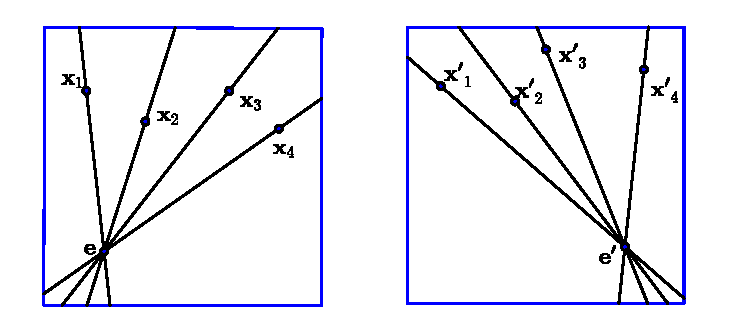
\includegraphics[scale=.85]{retas-epipolares}
\caption{\textit{Feixe de retas passando pelo epipolo em cada imagem, relacionadas duas a duas por uma homografia.}}
\label{retas-epipolares}
\end{figure}

Para a correspondência entre duas cônicas ${\bf \omega}$ e ${\bf \omega'}$ podemos utilizar a restriçao \textit{Kruppa}: as duas retas tangentes à ${\bf \omega}$ e passando por ${\bf e}$, estão relacionadas por uma homografia de reta epipolar às duas tangentes à ${\bf \omega'}$ passando por ${\bf e'}$. Na figura \ref{epipolar-kruppa} podemos visualizar as restrições epipolar e Kruppa simultaneamente.

\begin{figure}[!htb]
\centering
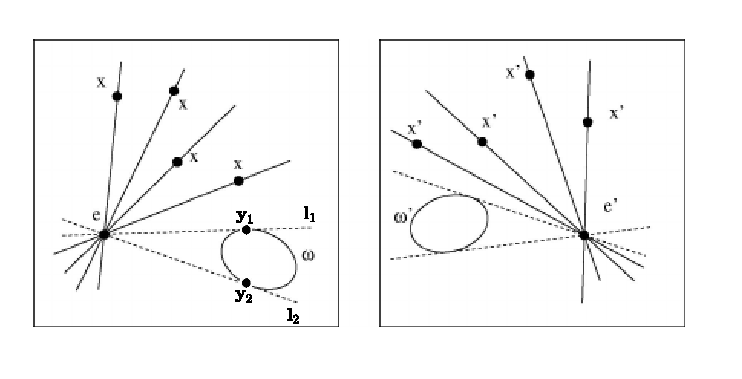
\includegraphics[scale=.85]{restricao-epipolar-kruppa}
\caption{\textit{Retas epipolares tangentes às cônicas ${\bf \omega}$ e ${\bf \omega'}$.}}
\label{epipolar-kruppa}
\end{figure}

De acordo com (semple e kneebone, 1952), podemos escolher as coordenadas projetivas de forma que os quatro pontos tenham as mesmas coordenadas em cada imagem. Ou seja, podemos assumir que ${\bf x}_i = {\bf x'}_i$ pensando nos dois planos de imagem como registrados no mesmo sistema de coordenadas. Desta forma, a restrição epipolar pode ser convertida em: os epipolos ${\bf e}$ e ${\bf e'}$, que obedecem a restrição epipolar, devem estar alojados numa cônica $B$ e, reciprocamente, dois epipolos ${\bf e}$ e ${\bf e'}$ que são concônicos com quatro pontos na imagem podem satisfazer a restrição epipolar. Esta cônica $B$ será bastante importante durante a abordagem pois, se os dois epipolos são concônicos com os quatro pontos na imagem, figura \ref{pontos-conconicos}, existe uma \textit{única} homografia de reta epipolar que faça a relação das quatro retas através ${\bf e}$ com as quatro retas através ${\bf e'}$. 

\begin{figure}[!htb]
\centering
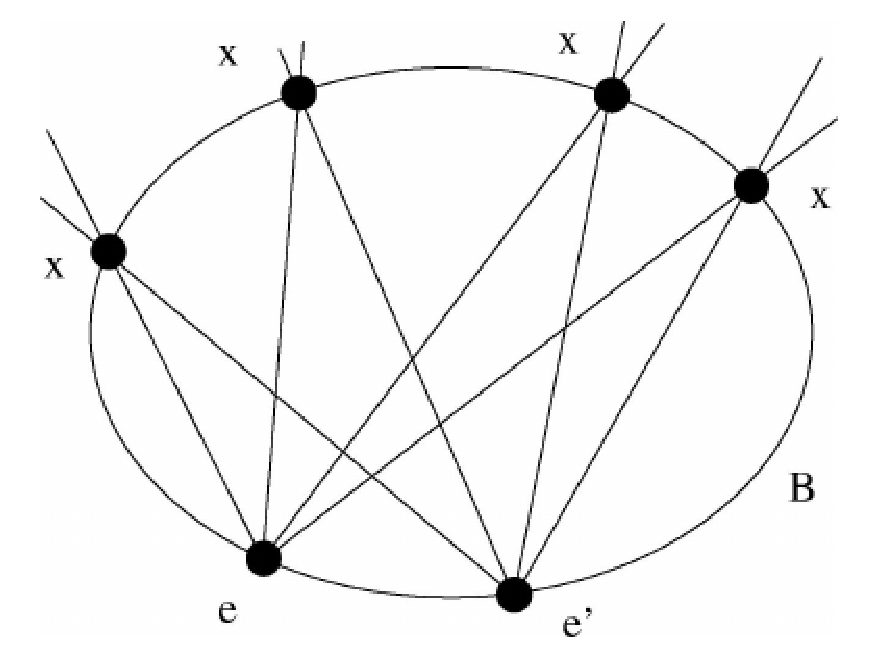
\includegraphics[scale=.85]{pontos-conconicos}
\caption{\textit{Epipolos concônicos com os quatro pontos na imagem produzem homografia única.}}
\label{pontos-conconicos}
\end{figure}

Note que podemos parametrizar o feixe de retas passando por ${\bf e'}$ (ou ${\bf e}$) por pontos pertencentes à cônica $B$, pois retas correspondentes nos dois feixes intersectam $B$ no mesmo ponto. Desta forma, a restrição Kruppa pode ser traduzida como: as restrições de calibração são equivalentes à condição de que as duas retas tangentes à cônica ${\bf \omega}$ e passando por ${\bf e}$, intersectam a cônica $B$ nos mesmos dois pontos adicionais que as retas tangentes à ${\bf \omega'}$ e passando por ${\bf e'}$. Isto é, as projeções de ${\bf \omega}$ e ${\bf \omega'}$ em $B$, através dos respectivos epipolos, devem coincidir. Essa construção geométrica pode ser visualizada na figura \ref{omega-B} e será a fundação para o resto da abordagem. 

\begin{figure}[!htb]
\centering
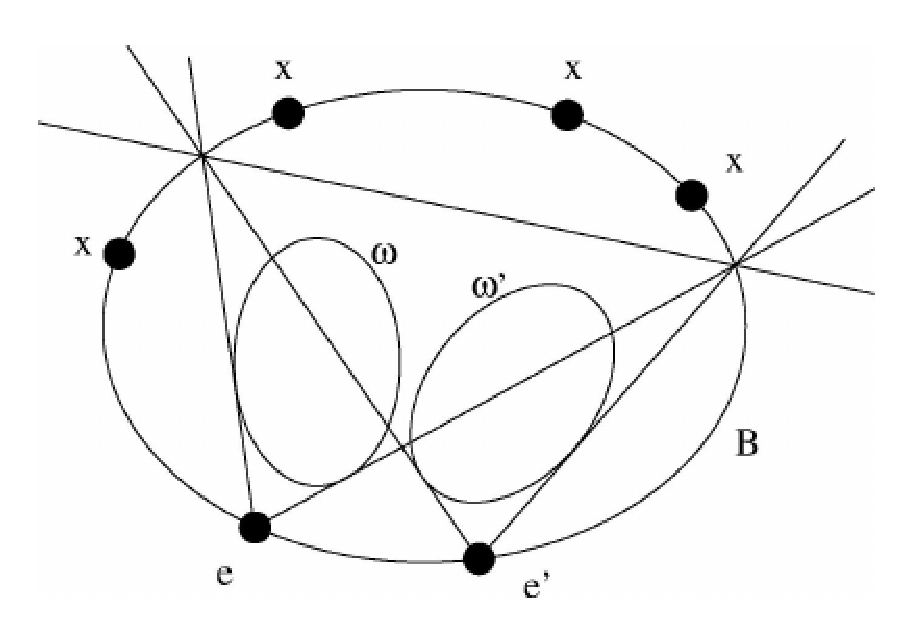
\includegraphics[scale=.85]{projecao-omega-B}
\caption{\textit{Os pontos de interseção das tangentes com a cônica $B$ coincidem, ocasionando a coincidência das projeções das cônicas ${\bf \omega}$ e ${\bf \omega'}$ na cônica $B$.}}
\label{omega-B}
\end{figure}

Podemos pensar na representação da projeção de  ${\bf \omega}$ e ${\bf \omega'}$ em $B$ como a reta que liga os dois pontos de interseção das tangentes com $B$. Essa reta que liga os dois pontos de interseção, de acordo com a projeção de ${\bf \omega}$ através do epipolo ${\bf e}$ é representada por $({\bf \omega}\diamond B)\,{\bf e}$, e a cônica $({\bf \omega}\diamond B)$ é definida como:

\begin{equation}
(\omega \diamond B)\equiv 2\,B\,\omega^*B - tr(\omega^*\,B)\,B,
\end{equation}
onde $\omega^*$ é a matriz adjunta de $\omega$.

Note que a reta $(\omega \diamond B)\,e$ é a reta polar de ${\bf e}$ com relação à cônica $(\omega \diamond B)$. Está sendo usada a relação polo-polar definida pelo locus da cônica $(\omega \diamond B)$ para executar a projeção. Já que os pontos de interseção das tangentes com $B$ são os mesmos para as duas cônicas $\omega$ e $\omega'$, pode ser verificado que, dado que ${\bf e}$ e ${\bf e'}$ são concônicos com quatro pontos na imagem, a restrição Kruppa é equivalente à restrição de que as retas polares $(\omega \diamond B)\,e$ e $(\omega' \diamond B)\,e'$ coincidem.


Note que $(\omega \diamond B) = B\,(\omega \cdot B)$ onde define-se a homografia

\begin{equation}
(\omega \cdot B) \equiv 2\,\omega^*\,B - tr(\omega^*\,B)\,I,
\end{equation}
onde está sendo ``cancelado" $B$ na definição de $(\omega \diamond B)$. 


Como $(\omega' \diamond B)\,e$ e $(\omega' \diamond B)\,e'$ coincidem e usando a equivalência anterior, pode-se demonstrar que 

\begin{equation}
(\omega' \cdot B)\,e' \sim (\omega \cdot B)\,e
\end{equation} 
(onde $\sim$ significa igualdade a menos da escala) o que implica num mapeamento de sétimo grau 

\begin{equation}
e \rightarrow e' \sim (\omega' \cdot B)^*\,(\omega \cdot B)\,e.
\end{equation}

No artigo também é domonstrado que a restrição Kruppa disponibiliza quatro soluções (dois pares de soluções coincidentes) para ${\bf e}$ para cada cônica $B$ e as soluções são as interseções (figura \ref{inter-B-C}) de $B$ com a cônica 

\begin{equation}
C \equiv (\omega \cdot B)^\top\,(\omega' \cdot B)^{*\,\top}\,B\,(\omega' \cdot B)^*(\omega \cdot B).
\end{equation}

\begin{figure}[!htb]
\centering
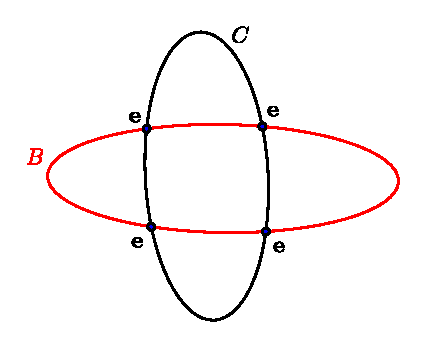
\includegraphics[scale=.6]{intersecao-C-B}
\caption{\textit{Epipolos que satisfazem as restrições de projeção e de calibração podem ser encontrados como as interseções das cônicas B e C.}}
\label{inter-B-C}
\end{figure}

Um epipolo ${\bf e}$ que gera uma cônica $B$ satisfaz à equação de décimo-sexto grau

\begin{equation}
{\bf e}^\top\,C\,{\bf e} = 0
\label{dezesseis}
\end{equation}
se, somente se, ele satisfaz às restrições de projetividade e de calibração. No caso em que a cônica $B$ pode se degenerar em um par de retas, a homografia $(\omega \cdot B)$ permuta as retas do par e assim, a equação \ref{dezesseis} descreve também seis retas passando por cada par dos quatro possíveis epipolos na imagem. Algebricamente, isso significa que a equação \ref{dezesseis} tem $|B|$ como um fator. Na figura \ref{plot-C} podemos observar duas plotagens da curva de dezesseis graus, uma com e outra sem a visualização dessas seis retas.

\begin{figure}[!htb]
\centering
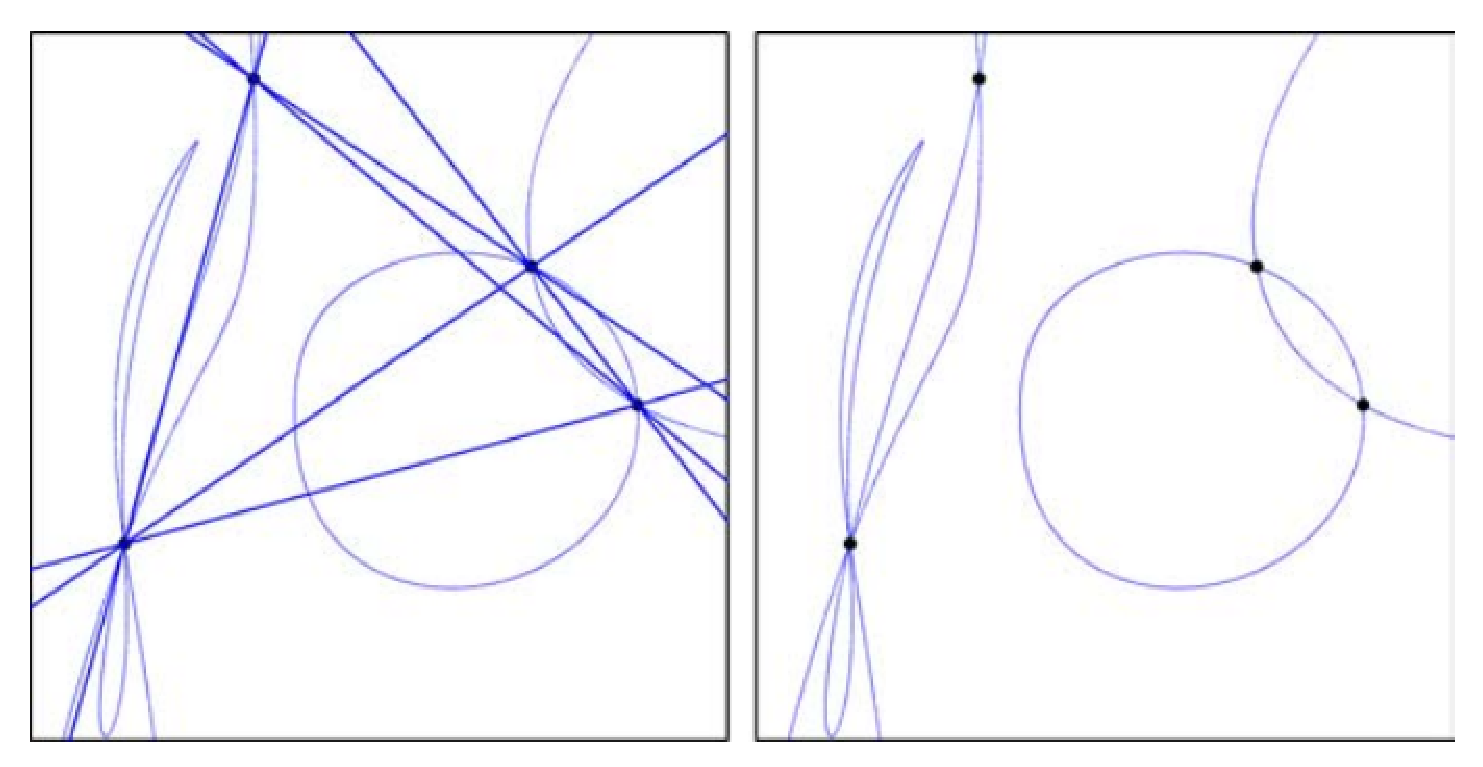
\includegraphics[scale=.6]{plotagem-C}
\caption{\textit{Podemos observar o lugar geométrico dos possíveis epipolos definido pela equação de décimo-sexto grau, juntamente com as possíveis seis retas.}}
\label{plot-C}
\end{figure}





\subsubsection{Abordagem de Schimd e Zisserman}

Este artigo lida com o problema de encontrar correpondências entre seguimentos de curvas quando temos diponíveis duas ou três imagens de câmeras deconhecidas. A matriz fundamental e o tensor trifocal são facilmente computados através de pontos de interesse mais o uso do RANSAC, mas os parâmetros intrínsecos não precisam necessariamente ser conhecidos. A abordagem clássica é descartar esses pontos de interesse e usar a geometria da câmera em estágios subsequentes de associação estéreo, para eliminar a ambiguidade entre pontos correspondentes ao longo da linha epipolar. Com duas imagens, o método padrão é usar a restrição epipolar para computar pontos correspondentes, o qual limita os canditados a estarem numa região estreita, e o uso de correleção cruzada normalizada, obtida a partir de fotometria, para restringir mais ainda nossas escolhas dos pontos. 

No artigo são analisados dois casos, binocular e trinocular, para responder a uma questão principal: existe alguma restrição adicional quando não utilizamos pontos mais sim pontos-tangentes ou geometria de curvas em geral disponíveis?\\

\noindent {\bf O Caso Binocular}

A busca por correspondências usando correlação fotométrica pode ser significantemente reduzida usando geometria de curvas (sem a utilização de contornos oclusos) numa pequena vizinhança. Considere uma aproximação de primeira ordem (planar) para a superfície de um objeto no qual aloja-se uma curva 3D. A correspondência entre as projeções desse plano em duas imagens são descritas por uma homografia de 8 parâmetros livres. É sabido que a matriz fundamental, que contém informações da geometria epipolar, fornece 5 restrições, o que reduz para 3 os graus de liberdade da homografia. Assim, o fato de que um ponto está associado a um outro ponto na reta epipolar já está sendo considerado nos cálculos. Dados alguns pontos correspondentes num fragmento de curva ao longo da linha epipolar, cada par de correspondência fornece duas restrições nas variáveis desconhecidas: como as curvas devem ser mapeadas umas nas outras, (i) a posição ao longo da linha epipolar define uma variável, já que o plano 3D é forçado a passar pelo ponto 3D reconstruído a partir dessa informação (a menos de uma homografia 3D). Assim, resta uma família de um parâmetro que pode ser otimizado usando o grau da correlação fotométrica. Dentre a família de um parâmetro de solução restante, os autores propuseram que, no lugar de otimizar através de correlação fotométrica, podemos apenas escolher o plano que coincide com o plano osculante da curva, o qual pode ser determinado usando a curvatura dos pontos correspondentes. Isto é apenas uma heurística, um método construtivo, onde não há garantia de que se trata da tangente à superfície, mesmo se a curva é plana. Contudo, empiricamente os autores expuseram que essa solução é boa o suficiente para criar uma fila ordenada das associações mesmo considerando os casos acima.

A questão de como conseguir um plano osculante (e a homografia associada a ele) foi a motivação para chegar a um resultado de interesse geral. Sabemos, através da posição e curvatura das extremidades correspondentes em duas imagens, que é possível estimar, unicamente, o plano osculante a uma curva se a calibração da imagem é completamente conhecida. Se apenas a matriz fundamental é conhecida, o plano osculante pode ser encontrado a menos da ambiguidade projetiva somente, mas a homografia associada a ele pode ser completamente determinada, o que é estudado nesse artigo.

\noindent {\bf O Caso Trinocular}

Os autores também propuseram um método para transferir a curvatura de duas imagens para uma terceira, dado um tensor trifocal (a calibração completa não é necessária). A interpretação da fórmula dada é usar o plano reconstruído a partir de duas imagens (conhecido a menos de uma ambiguidade projetiva 3D), e usá-lo para conseguir uma homografia relacionando as duas primeiras imagens com a terceira (sendo esta homografia independente dos parâmetros intrínsecos). Esta homografia define, então, a correspondência de pontos de quaisquer das duas primeiras imagens para a terceira. Faugeras e Robert foram os primeiros a proporem a transferência de curvatura a partir de duas imagens não calibradas para uma terceira, mas eles usaram par de matrizes fundamentais. O enriquecimento adicionado ao método de Faugeras proposto por Chimd e Zisserman é numericamente estável e imune a erros na interseção de linhas epipolares, que podem ser colineares ou aproximadamente colineares. O tensor trifocal manipula esses casos sem qualquer imprecisão.\\

\noindent {\bf Passo para um Sistema Prático} 

\begin{itemize}
\item Começar com a detecção de extremidades relacionadas em duas ou três imagens, e tentar associar fragmentos de curvas por inteiros.
\item Num primeiro estágio, considere apenas curvas alojadas no raio das linhas epipolares de cada uma das outras curvas, e têm tangências epipolares consistentes.
\item Num segundo estágio, tente encontrar fragmentos correspondentes de supostas curvas correspondentes através da integração do custo de extremidade-a-extremidade com possibilidade de associar fragmentos.
\item Usando apenas a geometria diferencial de curvas ganha-se restrições através de supostas extremidades associadas na terceira imagem. Isto funciona mesmo quando os parâmetros intrínsecos são desconhecidos, mas a ambiguidade permanece.
\item Restrições adicionais podem ser encontradas usando as aparências.
\item Para cada suposta associação, encontre um grupo de correlações no espaço gerado por um parâmetro se as curvaturas das associações são poucas (somente tangentes são utilizadas), ou não use buscas (planos osculantes) se as curvaturas acima são limites.
\item Um esquema das melhores escolhas dentre todas direciona para as associações finais.
\end{itemize}
